\chapter{Projet DN-Rider}
\label{chap:Projet DN-Rider}

\section{Constat \& Objectif du stage}
Objectif de ce project est de créer une application web (IHM + API REST) pour manipuler les notes de livraison Katana, elle va permettre de :

\begin{itemize}
  \item gérer l'objet NDL de manière plus simple qu'avec nexus/filesystème
  \item éviter les tableaux de suivi, type notes d'installation / tableaux de dépendances / ..., édités manuellement
  \item fédérer certaines fonctionnalités (extraction d'information, identification des package a installer sur une plateforme...) par rapport aux scripts bash/groovy/perl/ruby....
  \item  outiller le suivi du cycle de vie des versions par rapports aux infos remontées par les outils de l'usine logicielle et Katana
\end{itemize}

L’application devra être légère, dynamique et facilement évolutive, et non-contraignante pour les équipes.

Le but est de fiabiliser le processus de livraison et de mise en production des applications.
\clearpage

\section{Contexte \& Démarche}
\subsection{Contexte -- Equipe Intégration, Accompagnement Projet (transverse)}
Le project se déroule dans une équipe d'intégration. Le project est cadré par mon encadrant de stage qui désigne les objectifs du project. Pour le réaliser, je suis en accompagné d'un rérérent technique.

On a une organisation tranverse, le travail est autonomie, mais je le support de toute l'équipe.

\subsection{Démarche agile - devops}
Au sein de la VSCT, on met beaucoup de points sur la méthode agile et la discipiline "Devops". Dans cet équipe, on applique un "Kanban" pour l'organisation des travaux.  Comme sur la figure (fig. \ref{fig:kanban}), chaque membre dispose d'une lighe sur le tableau et chaque ligne est découpé en trois parties: "TODO", "EN-COUR" et "DONE" qui correspondant aux tâches à faire, tâche en train de faire et tâches réalisés. Les esapces laissées à gauche sont pour des idées qu'on va pêut-être planifier un jour.

\begin{figure}[h]
\centering
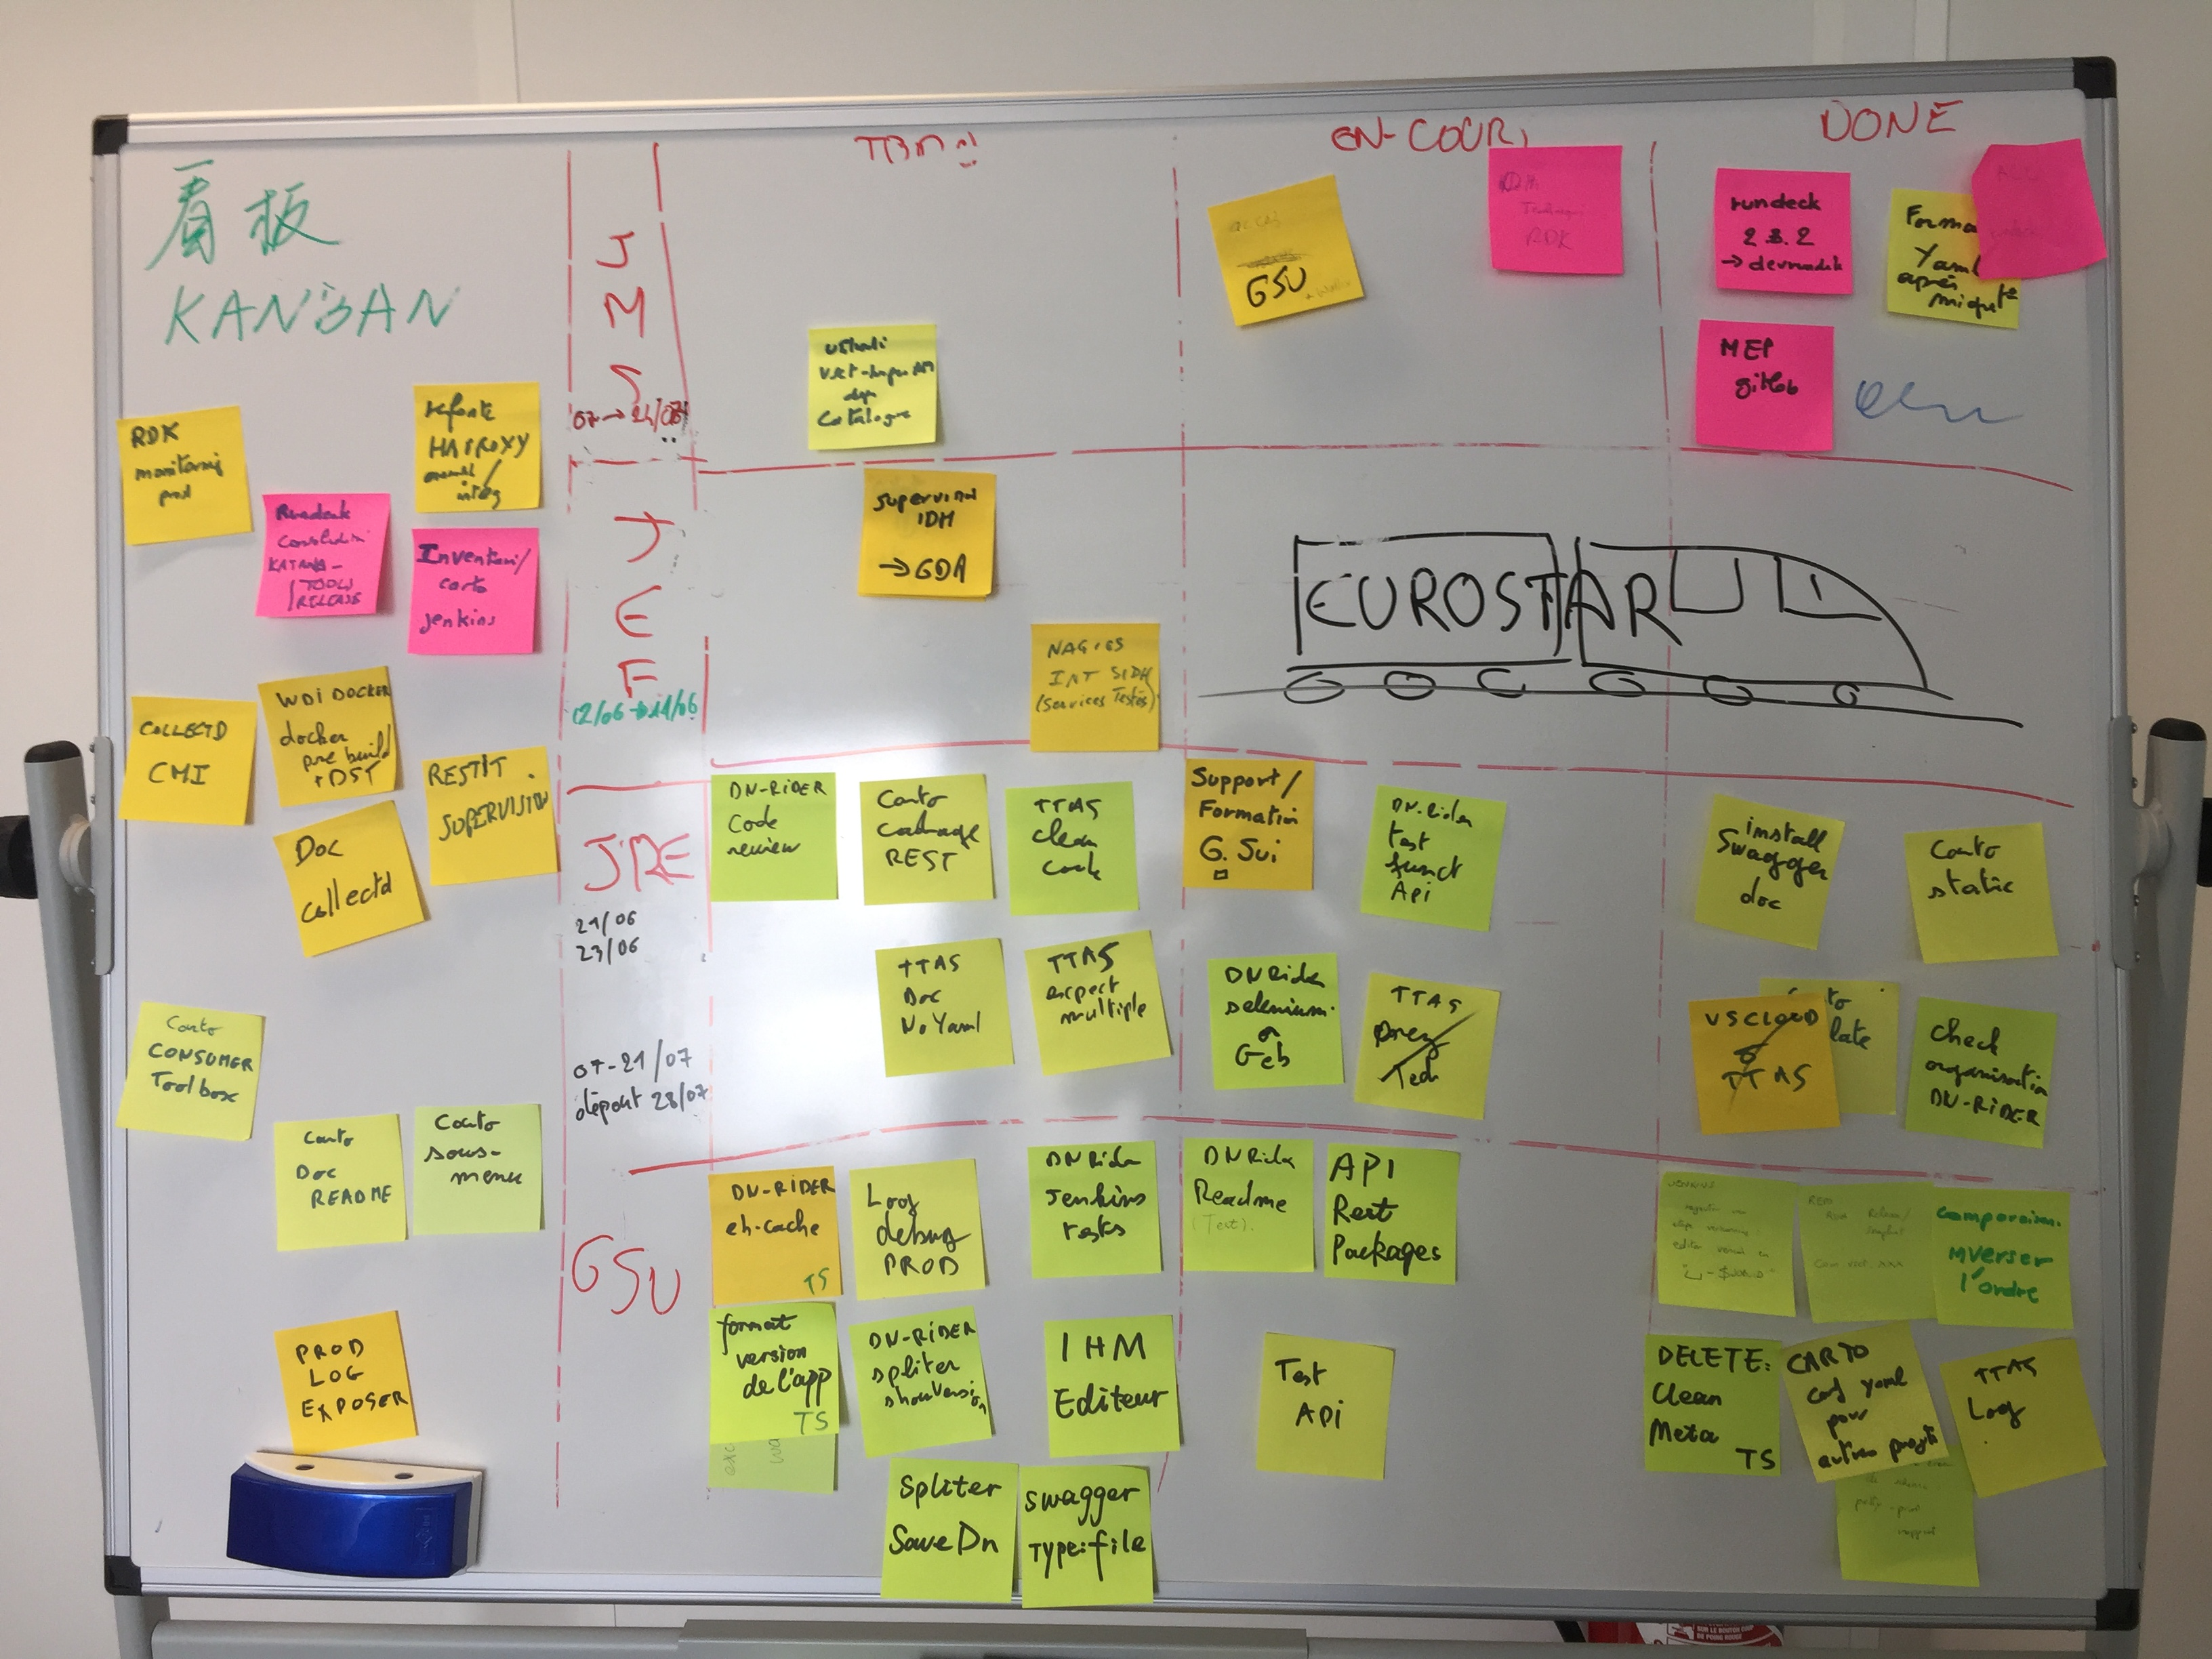
\includegraphics[width=0.8\textwidth]{kanban}
\caption{Kanban}
\label{fig:kanban}
\end{figure}

Les post-its sont classés par leur coleurs, les plus profonds correspondants aux tâches plus importants. Certains cartes sont marqué 'TS'(Technic Story) dessus, c'est-à-dire que c'est un petit sourcis technique qui est pas urgent à être résolu, on a une grande liberté de l'organiser seloon notre convenience.

Normalement on fait  deux fois par semine le review du Kanban pour garder le rythme. Chaque fois mes tuteurs valident ce que j'ai realisé et m'aident à planifier les tâches suivantes.

Les cods sources sont géré en git et stocké sur Gitlab. Au bout d'un mois et demi, on a la permière version de l'application et on commence à faire intégration continue en utilisant Jenkins pipeline. Chaque fois qu'il y a un commit sur la branche master, l'application seront déploié toutes seule.

\clearpage

\section{Application}
\subsection{présentation:}
IHM
Api REST(swagger)
Continus Delivery(git, test unitaire, pipeline->deploiement auto)

\subsection{Choix des technologies:}
Grails: référent compétent
Groovy:
Bootstrap:
Jquery:
Backlog:

\subsection{archi appli}
modèle MVC
lien vers Nexus

\clearpage

\section{Etat fin de stage}
\paragraph{1 application opérationnelle sur serveur PROD}
\paragraph{démo au sein de l’équipe (FUTUR démo global)}
\paragraph{bilan objectif de l’appli}

\clearpage
